
\setchapterpreamble[u]{\margintoc}
\chapter{Detection of archaeological remains with thermal imaging}
\labch{castle_puerta_arenas}
\label{sec:castle_puerta_arenas}

\section*{About this chapter}

This chapter describes the automatic reconstruction of thermal products depicting archaeological remains from the so-called Castle of Arenas (Jaén). These results are further analyzed to identify anomalies that may shed some light on remains that are still undiscovered. Despite these being visible on thermal reconstructions, the process was automatized in 3D with a voxelization that facilitated neighbourhood-based operations. The overall procedure of this work is shown in Figure \ref{fig:thermal_analysis_overview}.

\section{Historical background of Castle of Arenas}

The Arabic ruling in Spain started in 711, with the defeat of King Rodrigo in the Guadalete River. It had a huge development that only left a small reduct of Christians in the Northern mountains. From this Christian holdout, a reconquest was started that lasted eight centuries. The battle of Navas de Tolosa (Jaén) in 1212, also known as the battle of Al-Iqāb in Arabic historiography, was a key event for Christian kingdoms as part of the Spanish Reconquest. Most of the nowadays Andalusian lands fell to Christian forces, thus solely leaving the newly created Nasrid Kingdom of Granada, which had continuous changes in its boundaries. They finally surrendered to the Catholic Monarchs in 1492, and from this date, the entire Iberian peninsula was ruled by Christians. During this period, multiple defensive structures were built, changed and augmented, standing out those with a distinguished role for either part of the Reconquest. The Castle of Arenas, which is the main concern in this work, was one of these relevant fortresses. It is located over the top of a hill (Cerro del Castillo) at the end of the Alta Coloma mountain range. Therefore, the fortress has complete control over the valley of the Guadalbullón River. It is a calcareous gorge that forms a natural crossing of the East side of the Subbetica mountain range where several remains of previous ages have been found. Archaeological findings range from an Argaric passage-ritual area known as 'Puerta de Arenas', located in the South, to a Roman pavement in the North.

\begin{marginfigure}[-1.0cm]
    \centering
    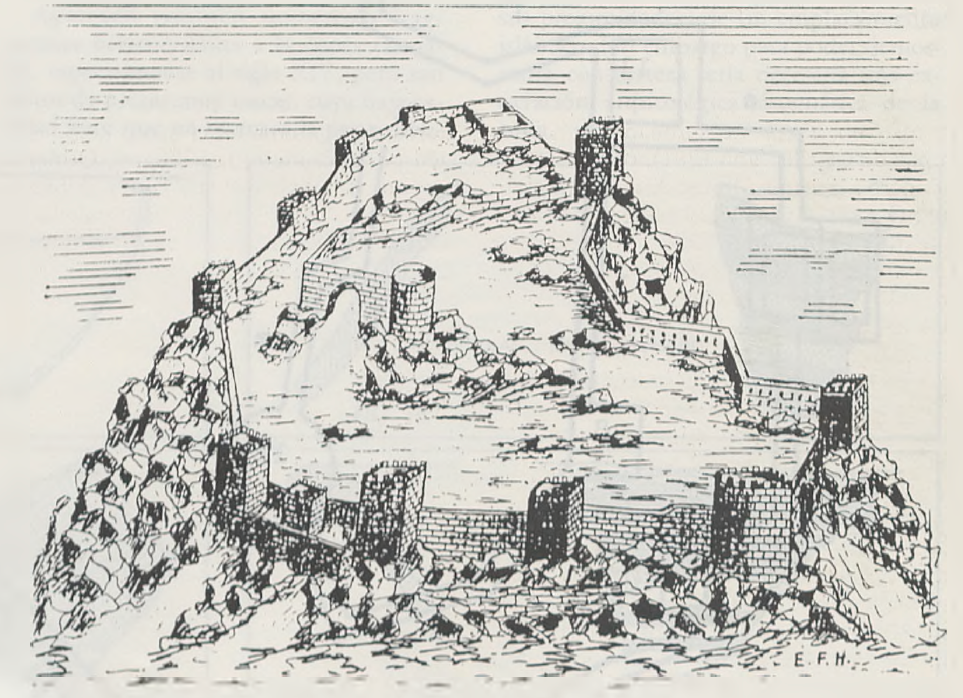
\includegraphics[width=\linewidth]{figs/castle_puerta_arenas/castle_ideation.PNG}
    \caption{Artistic ideation of the Castle of Arenas \cite{fernandez_hervas_castillo_1986}.}
    \label{fig:castle_ideation_art}
\end{marginfigure}
The Castle of Arenas originated under Arabic rule, though it may be possible that even a Roman fortress existed in this place \cite{fernandez_hervas_castillo_1986}. However, it was located at the boundaries between the Arabic Kingdom of Granada and the Castillian Kingdom, and therefore, it was part of both of them for centuries. It was first occupied by Fernando III in 1246, with the aim of recovering Jaén, though a few years later it was annexed to the Kingdom of Granada. Again, it was recovered by Alfonso X in 1280 and lost back in 1282 as the Castillian Kingdom trembled due to succession conflicts. This sequence was repeated over the next centuries: Alfonso XI pushed back the Arabic army to Granada in 1315, and it was only part of the Castillian Kingdom for four years. In the 14th century, several scuffles were attempted by Miguel Lucas de Iranzo to recover it from the Arabic kingdom. It was not until 1481 that the castle was again mentioned in some brief notes as part of the domains of Jaén.

The remains of the Castle of Arenas comprise a few towers and walls in a very steep mountainous location that makes it very hard to explore. Furthermore, it has been very poorly conserved in contrast to other notable Andalusian fortresses from the Arabic kingdoms. Most of the documentation found about this fortress was collected by Enrique Fernández Hervás in 1986 \cite{fernandez_hervas_castillo_1986}, while more recent explorations have been performed by Francisco Olivares \cite{olivares_castillos_1992}. The former depicted what was believed to be the shape of the castle (see Figure \ref{fig:castle_ideation_scheme}), where its main inaccuracies will be shown throughout this chapter by showing the aerial view. Although the main shape is inaccurate, some features were accurately represented and the errors were just the aftermath of ground-based observations.

\begin{figure}[ht]
  \centering
  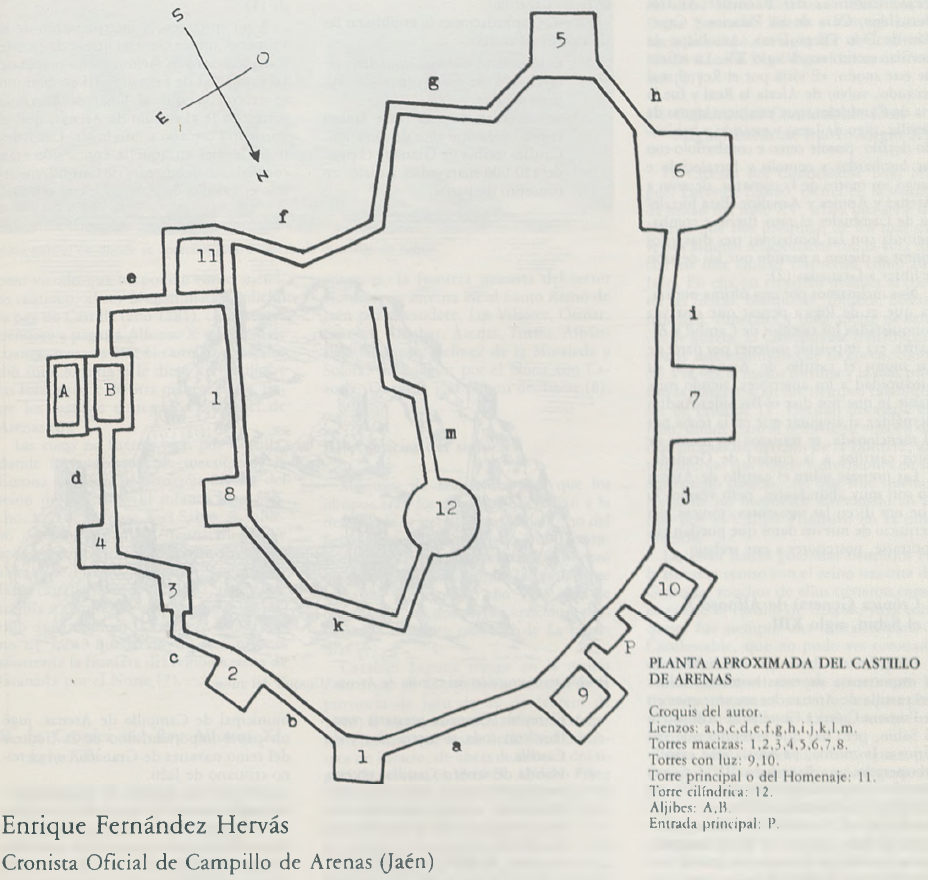
\includegraphics[width=\linewidth]{figs/castle_puerta_arenas/castle_ideation_scheme.PNG}
  \caption{Scheme of the structure of the Castle of Arenas, proposed by Enrique Fernández Hervás \cite{fernandez_hervas_castillo_1986}.}
  \label{fig:castle_ideation_scheme}
\end{figure}

\section{On the inspection of archaeological remains}

The preservation of cultural heritage has recently benefited from the use of high-resolution digital cameras that allow the reconstruction of a scenario with high precision. Aerial images acquired from drones not only allow us to generate 3D models using photogrammetric techniques but also to obtain information beyond the visible wavelengths depending on the coupled sensors. Thermal imagery has been widely explored to find archaeological remains since underlying structures interact with the foreground surface by transferring its temperature, which may be significantly different from the surroundings. From the literature, some of the most outstanding works are authored by Casana et al. \cite{casana_archaeological_2017} and Carmona et al. \cite{salgado_carmona_assessing_2020}, which successfully attempted to find buried remains of ancient civilizations. The energy transfer of thermal imagers is exhaustively described by Vollmer \cite{vollmer_infrared_2017}; however, a briefer summary of what thermal anomalies ought to be like in archaeological remains is explained by Casana et al. \cite{casana_archaeological_2017}, as depicted in Figure \ref{fig:thermal_transfer}. Also, this work showed how temperature varies throughout the day for different surfaces, and therefore, specific hours may be better than others to maximize the thermal contrast).

\begin{figure}[ht]
    \centering
    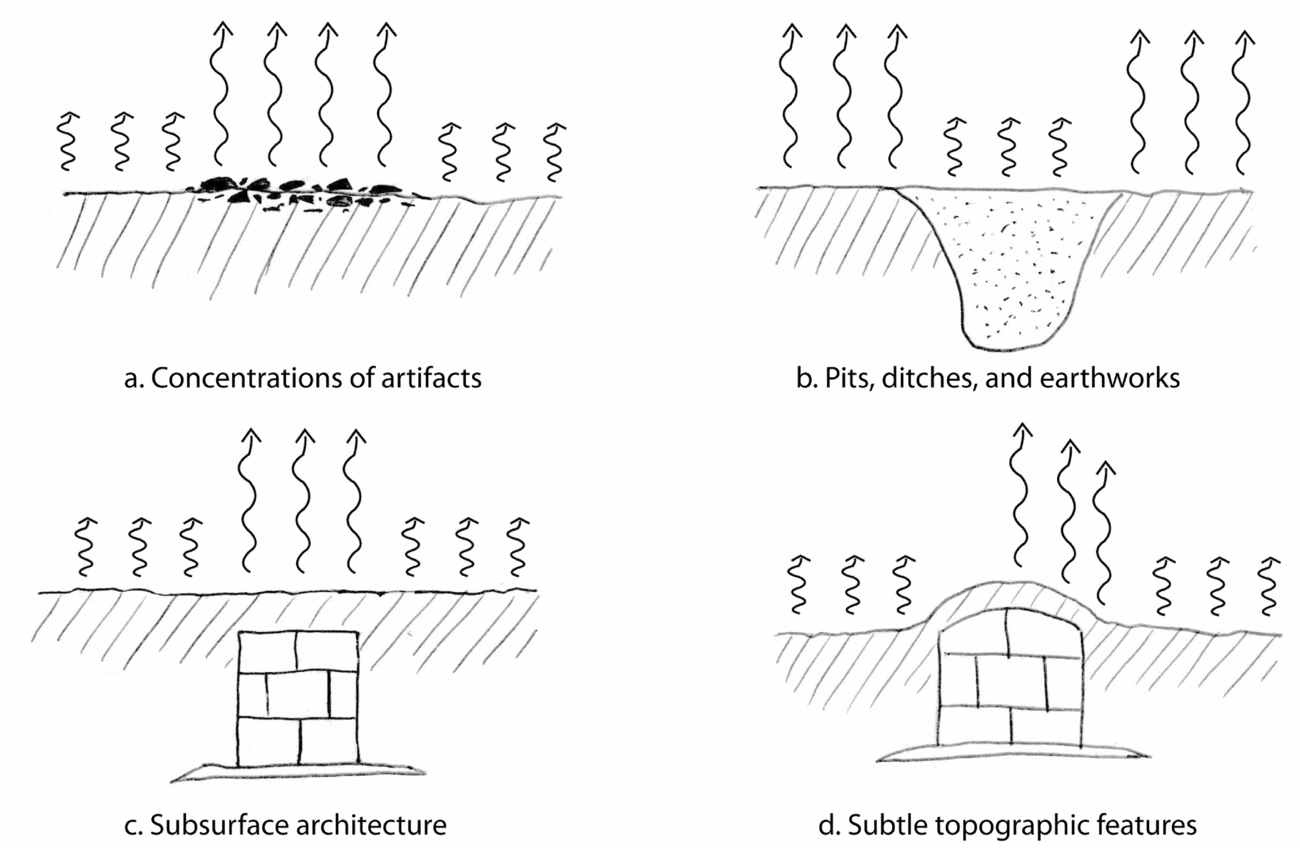
\includegraphics[width=\linewidth]{figs/castle_puerta_arenas/thermal_exchanging.png}
	\caption{Anomalies that could be observed in archaeological remains, according to if these are buried, visible or remains are simply variations in the ground compounds \cite{casana_archaeological_2017}.}
	\label{fig:thermal_transfer}
\end{figure}

In contrast to thermal imagery, visible sensors acquire images of higher resolution, enabling the estimation of larger and more dense point clouds. Accordingly, \acrshort{rgb} point clouds can be used as a constrained data source to map thermographic information, thus taking advantage of the spatial characteristics. For that purpose, the differences between visible and thermal imagery were estimated using \acrshort{ecc}, as explained in a previous chapter. The 3D thermal point cloud was estimated over an \acrshort{rgb} point cloud, using the previously computed matrices that allow projecting thermal imagery into \acrshort{rgb} data. Finally, a large number of 3D \acrshort{rgb} points were projected into \acrshort{rgb} (and thermal) imagery using the camera matrices estimated during the photogrammetric reconstruction. 

\begin{figure*}[htbp]
   \centering
    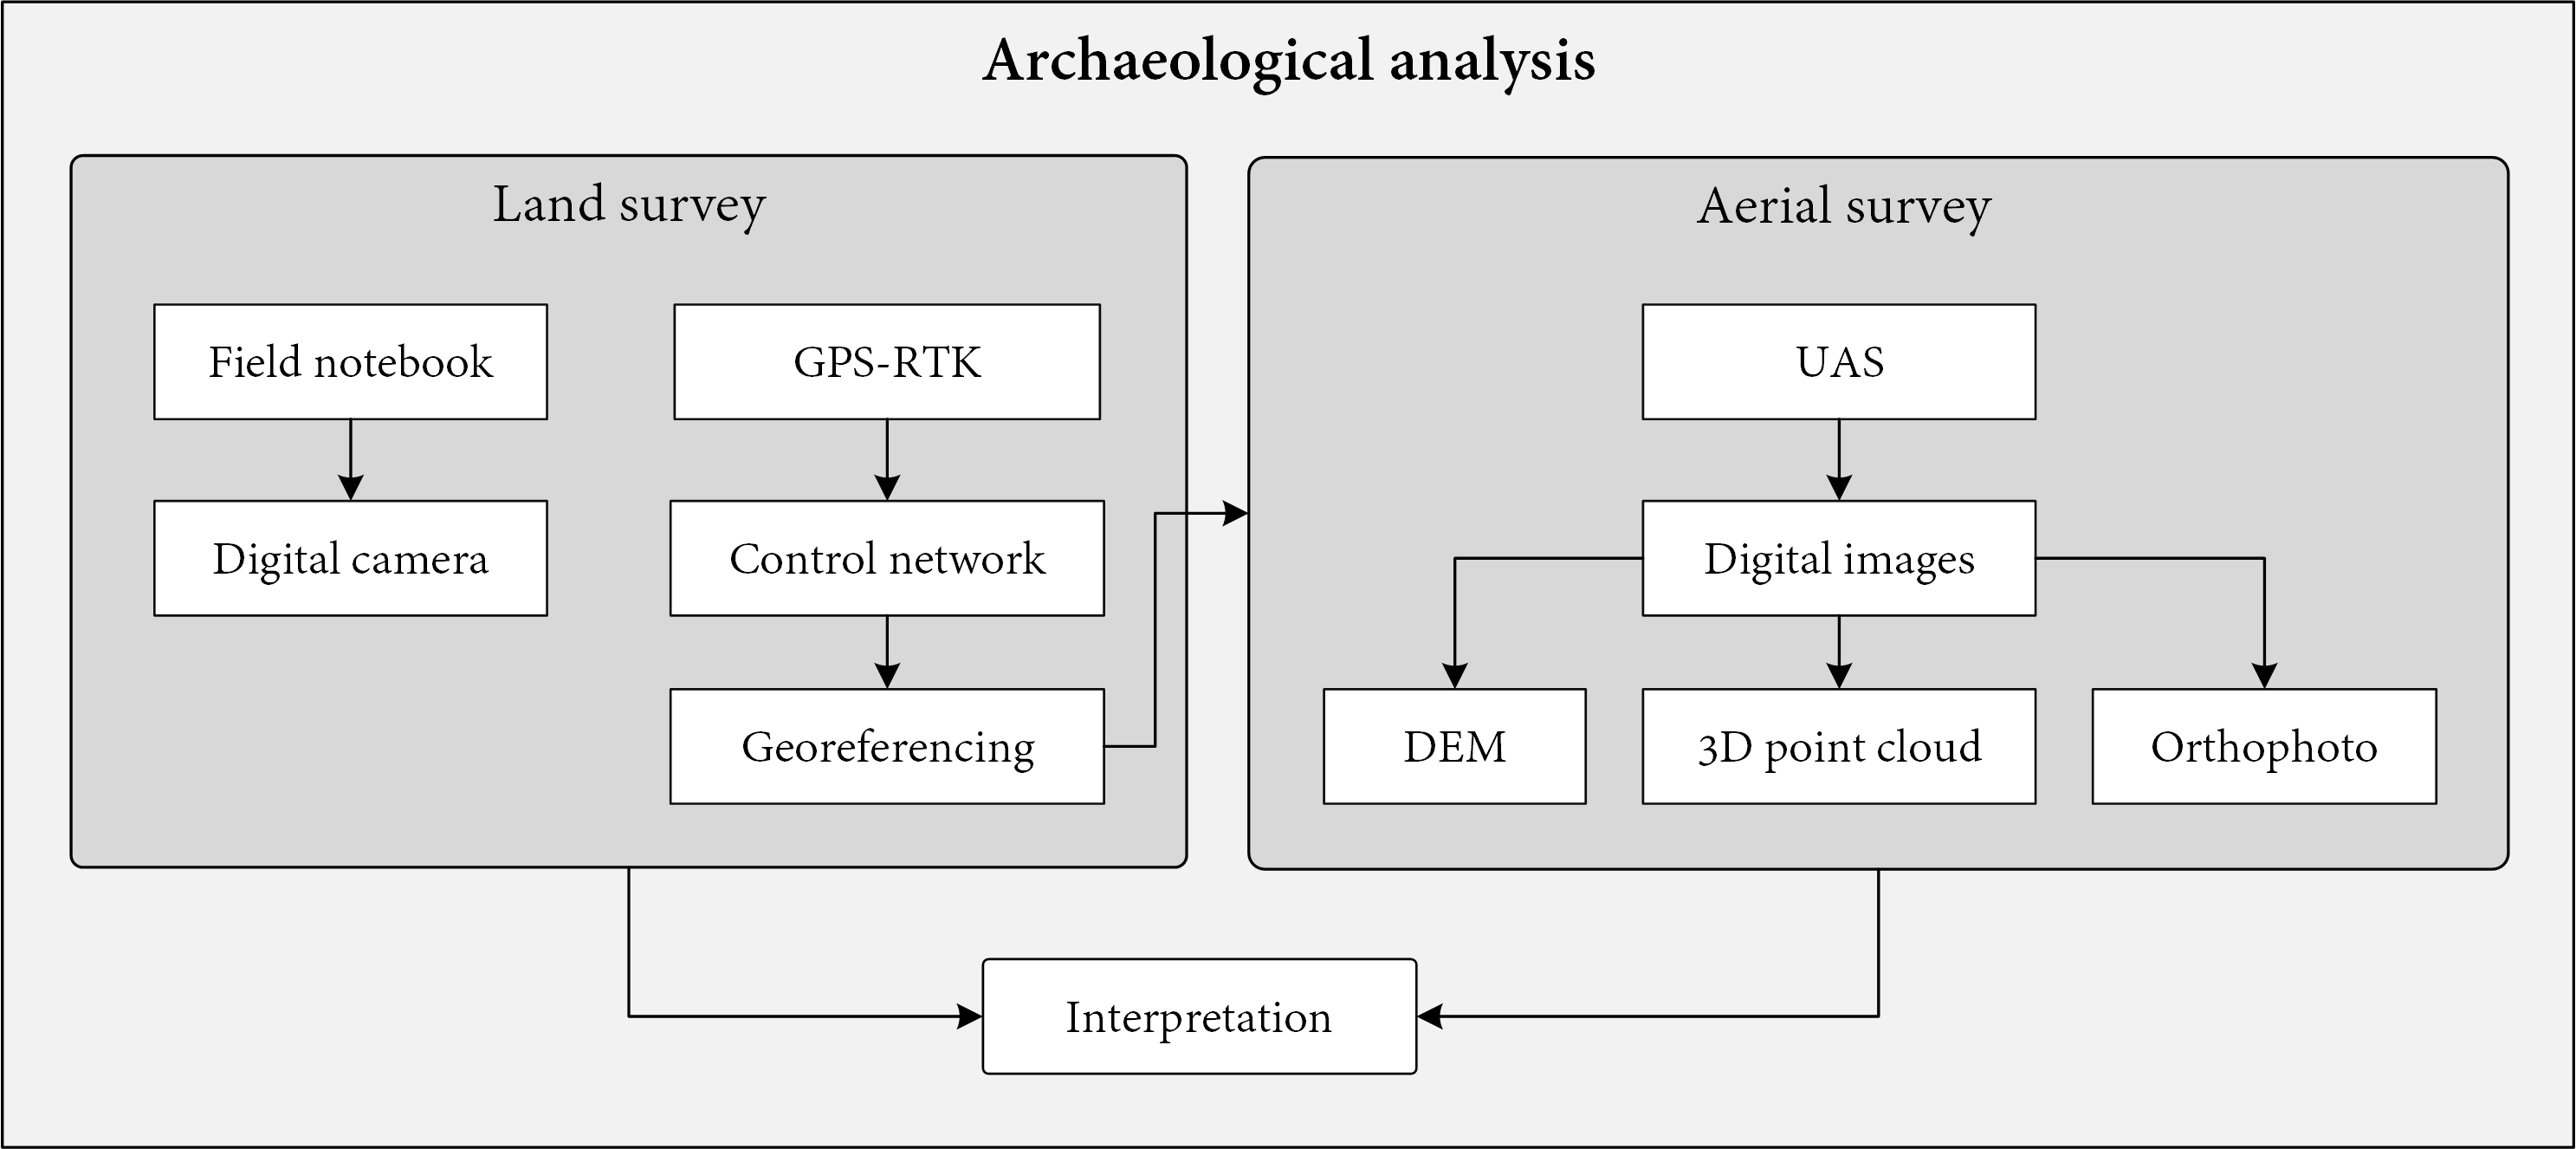
\includegraphics[width=\linewidth]{figs/castle_puerta_arenas/overview.png}
   \caption{Overview of the proposed methodology. The archaeological remains are monitored through land and aerial surveying. The first is simply used to help with the analysis from the latter survey, whereas the \acrshort{uas} results provide a better insight into details that could not be observed from land.}
   \label{fig:thermal_analysis_overview}
\end{figure*}

\section{Study area}

\begin{marginfigure}[-.8cm]
    \centering
    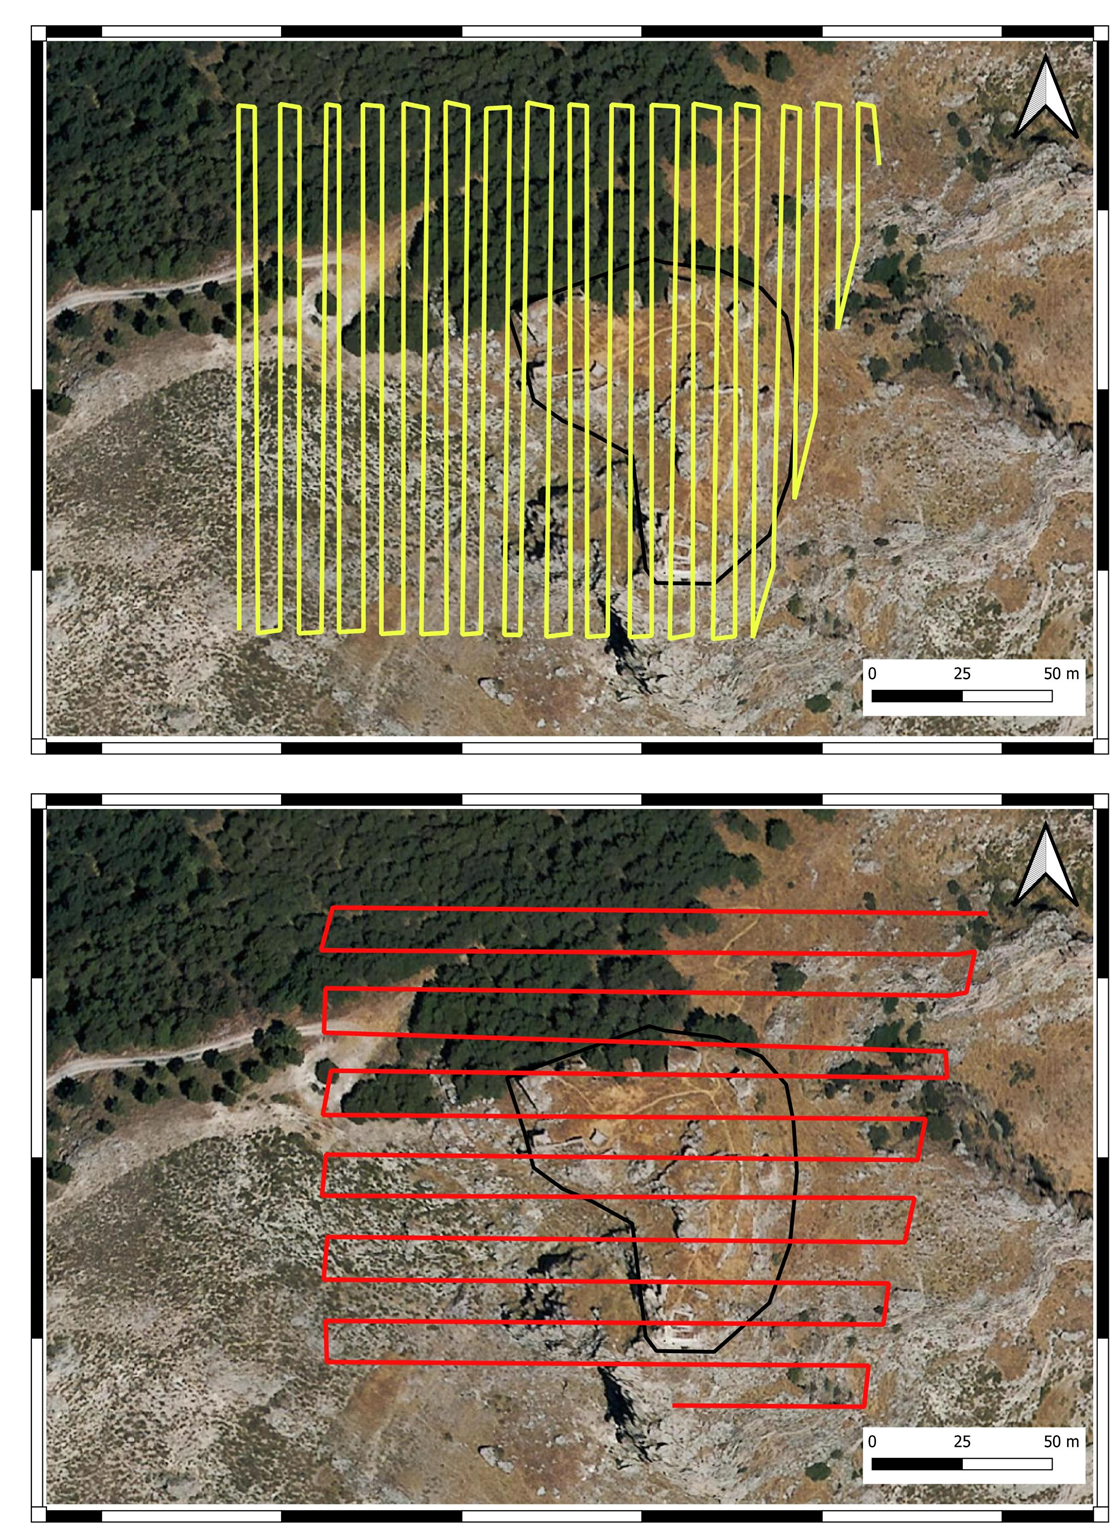
\includegraphics[width=\linewidth]{figs/castle_puerta_arenas/uav_paths.png}
    \caption{Path from two \acrshort{uas} flights performed with different forward directions to capture features from the fortress walls.}
    \label{fig:flight_paths}
\end{marginfigure}
The Castle of Arenas is located over a hill called Cerro del Castillo, 39 \si{\kilo\meter} at the South of Jaén. The geographic coordinates are $37^{\circ}35'34'' \hspace{1mm}$N and $3^{\circ}37'20'' \hspace{1mm}$WG following the ETRS89 reference system. The altitude is approximately 1370 \si{\meter} above sea level, with the summit placed at 1393 \si{\meter}, and the lower wall at 1360 \si{\meter}. The surveyed area covers about 0.6 \si{\hectare} depicted in Figure \ref{fig:study_site}. Four flights were performed according to the limited flight time ($\sim$90 \si{\minute}), including one \textit{nadir} and three oblique flights. The latter three were performed to observe wall features. Flights were carried out at an altitude of 60 \si{\meter} above ground level for the first one, and 50 \si{\meter} for the rest. The \acrshort{gsd} of the collected imagery was 2.1 \si{\centi\meter}/pixel and 6.0 \si{\centi\meter}/pixel for visible and thermal imagery, respectively. The flight was conducted close to midday in order to minimize shadows from the remains. This period was preferred over the period between sunset and sunrise due to safety reasons, despite the latter being more optimal for thermal surveys. The collected temperature for each flight is summarized in Figure \ref{fig:temp_histogram}. 

\begin{figure*}[htbp]
  \centering
  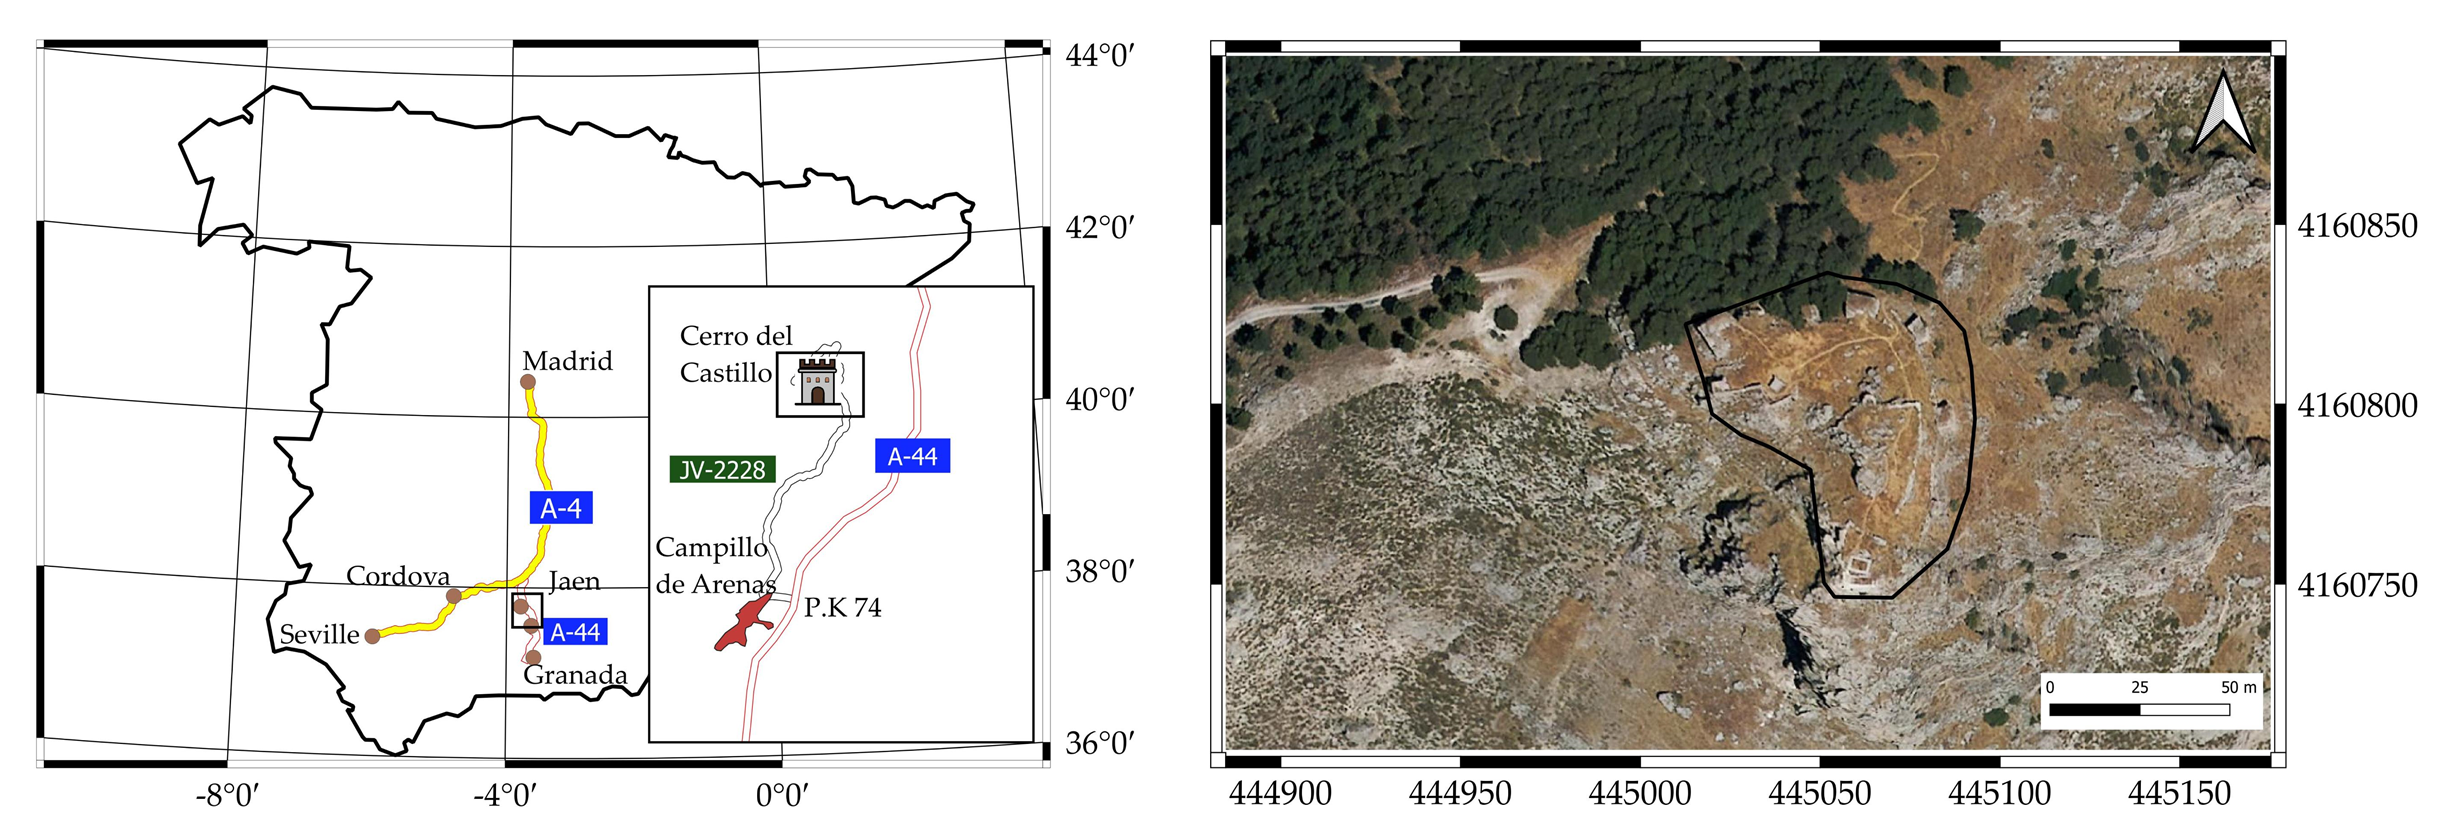
\includegraphics[width=.92\linewidth]{figs/castle_puerta_arenas/study_area.png}
  \caption{Overview of the research area. The right image shows the surveyed area, with the archaeological remains highlighted as a black polygon. The coordinates are in the \acrshort{utm} reference system (\si{\meter}), zone 30, ETRS89.}
  \label{fig:study_site}
\end{figure*}

\begin{figure}[ht]
    \centering
    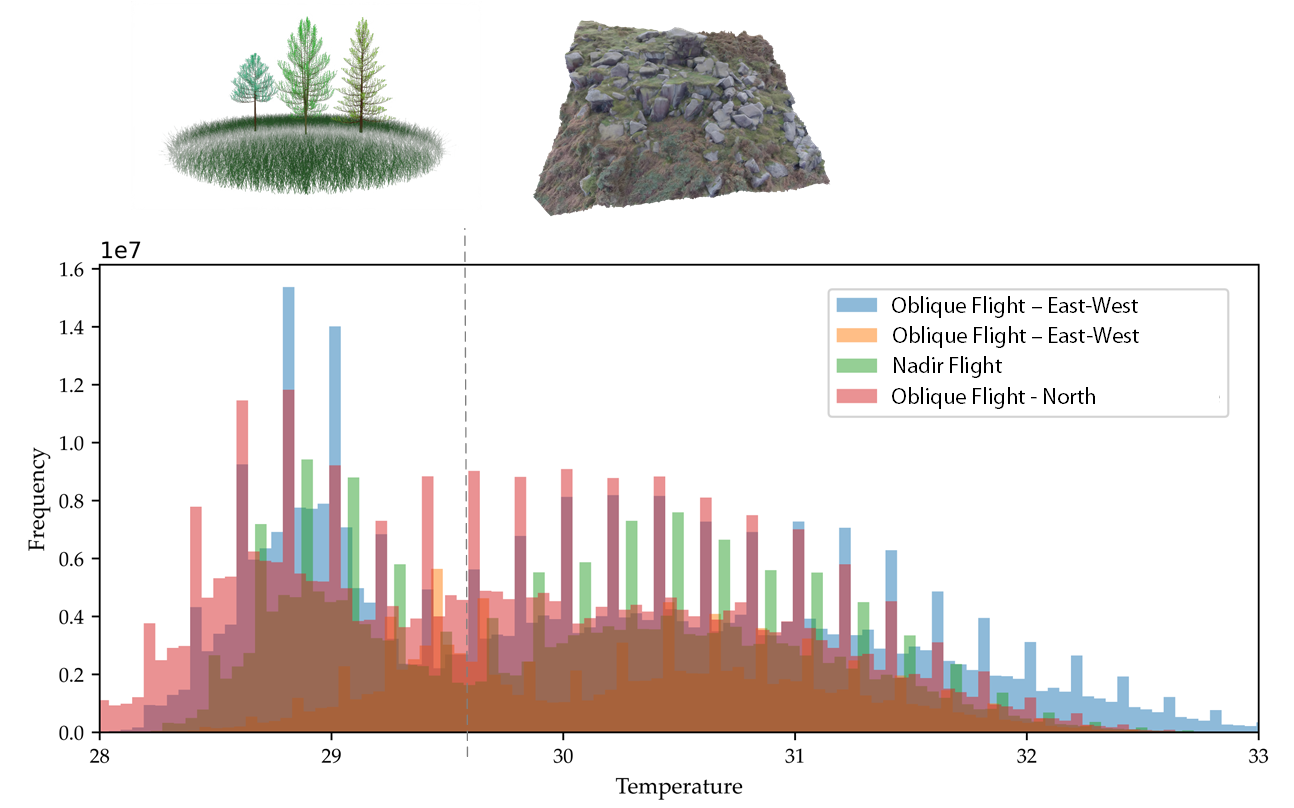
\includegraphics[width=.9\linewidth]{figs/castle_puerta_arenas/thermal_histogram.png}
	\caption{Histogram of radiometrically corrected thermal samples as collected for every flight. Lower temperature values may correspond to vegetation, whereas the centre is mainly linked to rock masses, either from archaeological features or not. Higher temperature is linked to anomalies and heated rock masses. }
	\label{fig:temp_histogram}
\end{figure}

\subsection{Acquisition of ground control points}

The first step in the acquisition of information is to obtain the coordinates of \acrshort{gcp}s, since they help to improve the accuracy and quality of later results. These coordinates were acquired using a couple of Topcon GR5 \acrshort{rtk}-\acrshort{gnss} in \acrshort{rtk} mode. The reference station was placed in the trigonometrical station of Orozco, which belongs to the REGENTE network, placed at 1120 \si{\meter} from our study area. According to the manufacturer specifications, the precision of East and North components is approximately 0.006 \si{\meter} (5 \si{\milli\meter} $\pm$ 0.5 \si{\milli\meter}), whereas the precision of the $\Vec{\textit{up}}$ component is about 0.011 \si{\meter} (10 \si{\milli\meter} $\pm$ 0.8 \si{\milli\meter}). Hence, the accuracy of these measurements was in the order of \si{\centi\meter}. The placement of the \acrshort{gcp}s was carefully designed to obtain results georeferenced in a national grid and height datum. From now on, coordinates will be displayed in meters (\si{\meter}), map projections will be depicted in the \acrshort{utm} system, the reference system will be the ETRS89 and altitudes will be calculated according to the mean sea level in Alicante, Spain. Six \acrshort{gcp}s were more likely to be enough due to the small size of the study area ($\sim$0.6 $\si{\hectare}^2$), although ten were finally acquired to capture the details of the steep orography. From these, only seven were used to georeference the images, whereas the rest were used as control points. Two of them were located at the side of the hill (1350 \si{\meter}).

The measured \acrshort{gcp}s allowed us to evaluate the accuracy of a 3D model in terms of scale. This was checked using the \acrshort{rmse} for the X, Y and Z axes, as defined in Equation (\ref{eq:thermal_analysis_rmse}). The acquisition of imagery and \acrshort{gcp}s are the baseline of our methodology. From here, 3D results are estimated to provide a better data source on which later visualization and analysis tasks are easier to perform by human operators.
\begin{equation}
\label{eq:thermal_analysis_rmse}
\textit{RMSE} = \sqrt{\frac{1}{n}\Sigma_{i=1}^{n}{\abs{P_{i} - P_{{i_{\textit{GNSS}}}}}^2}}
\end{equation}
where $P_{i_{\textit{GNSS}}}$ is the location of a \acrshort{gcp}, $P_{i}$ is the i-th point from a point cloud and $n$ is the number of pairs of points (\acrshort{gcp} and reference point). Table \ref{table:point_coordinates} shows an overview of the acquired \acrshort{gcp}s along with the estimated error and the \acrshort{rmse} concerning control points and checkpoints.

\section{Reconstruction of RGB point cloud}

The estimation of \acrshort{rgb} point clouds was conducted with the \acrshort{sfm} algorithm provided by Agisoft Metashape\textregistered (version 1.7.5). The 3D modelling of archaeological sites is usually carried out to evaluate them using a computer-based model, instead of the real-world one. In this regard, \acrshort{uas}s are a major breakthrough technology for increasing the knowledge of ancient civilizations. Some of the conditions taken into account, given that this work is focused on archaeology and thermal imaging, were to collect the data with sufficient light and to avoid a high downscaling during \acrshort{sfm} to ensure a high \acrshort{lod} and preserve most of the features.

\section{DEM and orthomosaic}

The following step is to generate the \acrshort{dem} with high quality (see Figure \ref{fig:thermal_castle_dem}). It also involves extracting the analytical hill shading, derivatives of hill-shading from different directions (range of hill shadings, mean of hill shadings and \acrshort{pca} of hill shadings), elevation differentiation, trend removal, slope severity, sky-view factor, solar insolation modelling, as well as composite images using the normalized \acrshort{dsm} and the shaded relief. The objective is to interpret the topography by means of visual features and slope variations, i.e., using a geomorphometric approach guided by the ground surface. 

\begin{figure*}[htbp]
    \centering
    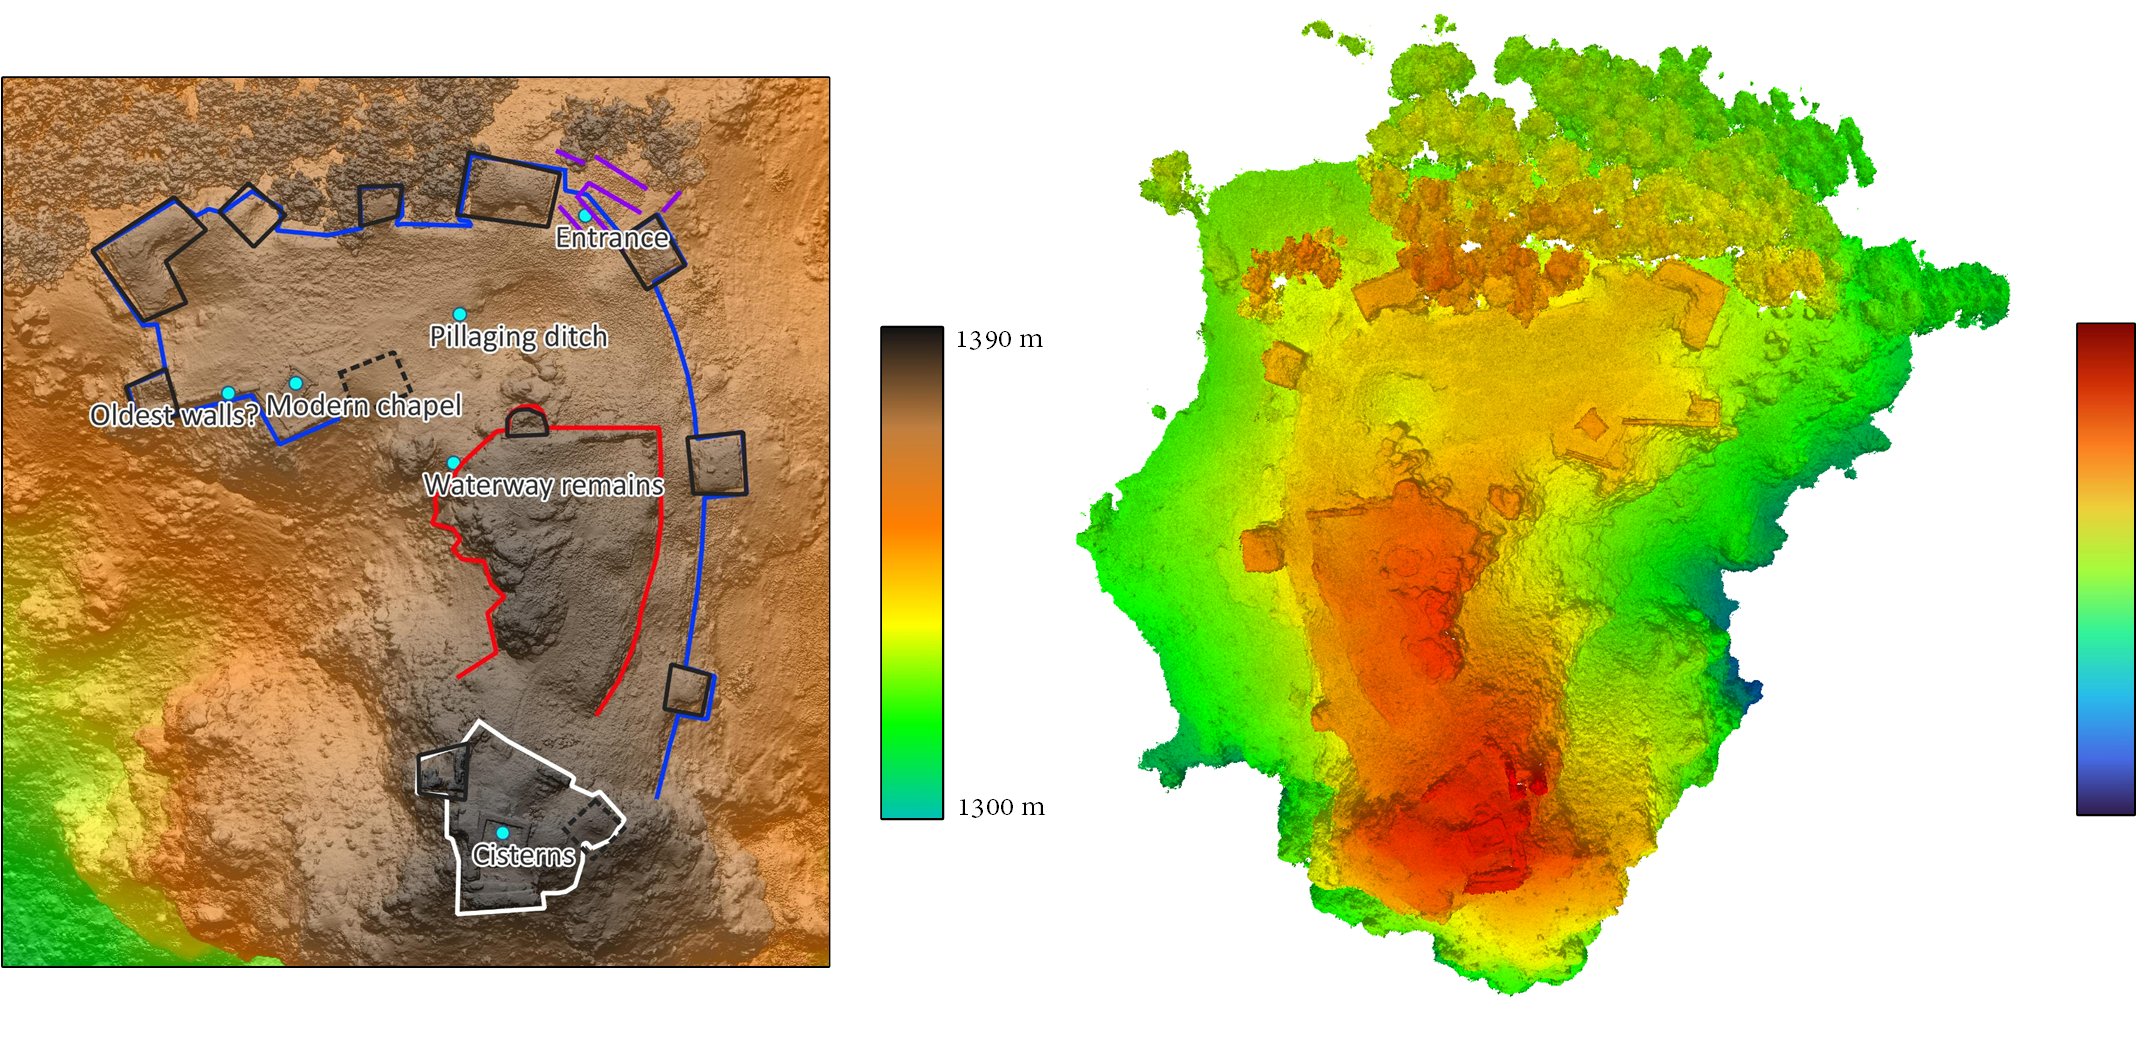
\includegraphics[width=\linewidth]{figs/castle_puerta_arenas/fortress_height.png}
    \caption{\acrshort{dem} of the fortress along with a point cloud shaded according to the relative height. }
    \label{fig:thermal_castle_dem}
\end{figure*}

\section{Thermal modelling}

The 3D thermal modelling of the surveyed environment is performed using the methodology described in Chapter \ref{sec:thermal_pc}. Briefly, thermographic data was projected into a dense \acrshort{rgb} point cloud of nearly 100 million points. Firstly, visible and infrared imagery were geometrically corrected and aligned to estimate the homography matrices that enable overlapping them. Then, camera matrices estimated during \acrshort{sfm} were used to project 3D \acrshort{rgb} points into \acrshort{rgb} imagery, and subsequently, to thermal imagery. The resulting thermal point clouds accumulate two layers: 1) grayscale infrared values, and 2) radiometrically corrected temperature, ranging from 28 \si{\celsius} to 33 \si{\celsius}. The latter is represented as an absolute value, in comparison with the greyscale representation.

\section{Anomaly detection}

\begin{marginfigure}[.2cm]
    \centering
    \includegraphics[width=\linewidth]{figs/castle_puerta_arenas/thermal_point_clouds.png}
	\caption{a) Thermal point cloud and b) fused rendering of \acrshort{rgb} and thermal point cloud to highlight statistical anomalies.}
	\label{fig:thermal_anomaly_detection_3d}
\end{marginfigure}
Despite outlier areas being visible over the thermal point cloud, their visualization can be enhanced by highlighting relevant features from the rest of the environment. This fusion of thermal and \acrshort{rgb} colours was already explained previously; the latter is fused with the first according to $w(t)$, which weighs how anomalous a sample ($t$) is. Thus, values are classified as anomalies whether they lie outside the interquartile range. Figure \ref{fig:thermal_anomaly_detection_3d} shows the rendering of the reconstructed thermal point cloud by combining both \acrshort{rgb} data and temperature to show outliers. Both of them highlight areas that are suspected to cover yet unknown remains of two different towers. 

These outliers can also be highlighted in 3D using infrared data from the surroundings. The main challenge is to efficiently find the neighbourhood. Although the benefits of using Morton encoding and sorting have been shown throughout this dissertation, it does not handle well spatial queries based on a radius since the notion of space is discarded at the expense of efficiently solving operations in a 1D buffer. Therefore, other trivial data structures, such as a regular grid (see Figure \ref{fig:voxel_anomalies_scheme}), seem more appropriate to solve neighbourhood searches with a complexity of $\mathcal{O}(1)$ (or $\mathcal{O}(n)$ whether a list of primitives is attached to every voxel). Hence, the thermal point cloud is discretized using voxels of a fixed size. It can be efficiently computed in the \acrshort{gpu} since points can be easily indexed into a voxel, whereas the memory footprint is parameterized by the voxel size.

\begin{figure}[ht]
    \centering
    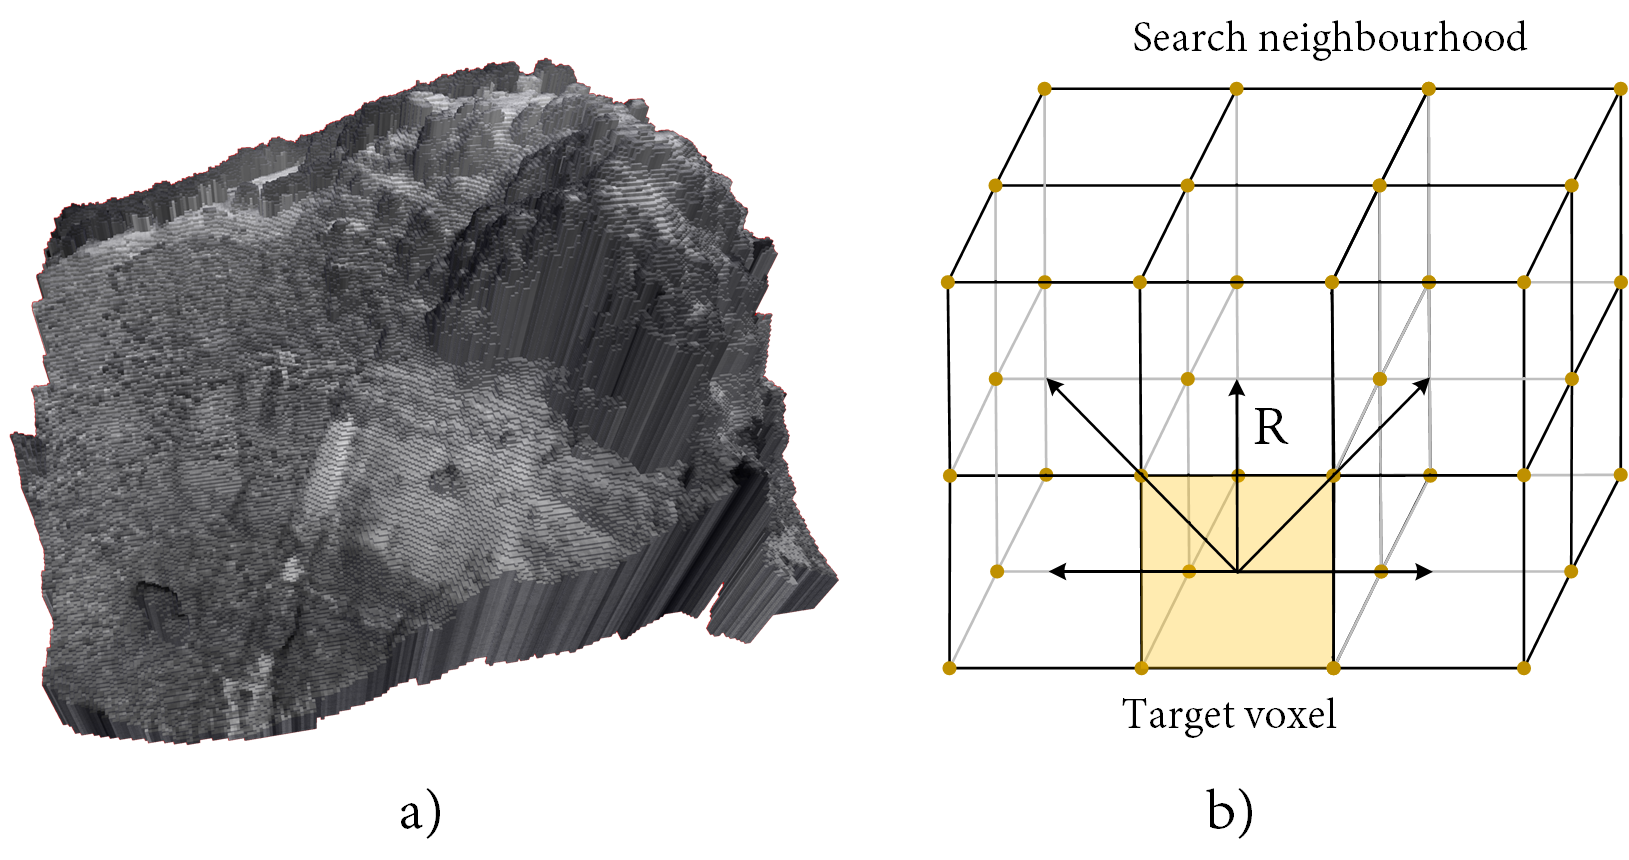
\includegraphics[width=\linewidth]{figs/castle_puerta_arenas/voxel_anomalies.png}
	\caption{Overview of the anomaly detection procedure. a) Voxelized environment, and b) neighbourhood of a voxel at a distance of $r$.}
	\label{fig:voxel_anomalies_scheme}
\end{figure}

\newpage
Following this approach, the point cloud was voxelized using a variable number of subdivisions, with each cell storing the average temperature of the included subset of points. Those voxels whose temperature is notably different from their surroundings are highlighted in the rendering. Accordingly, a voxel is marked as an outlier whether the temperature difference is above $\kappa \cdot \sigma$, provided that $\sigma$ represents the standard deviation of a neighbourhood, and $\kappa$ is a user-defined factor that can be interactively changed. Figure \ref{fig:voxel_anomalies} shows the thermal anomalies of a 3D voxelization of size $300 \times 150 \times 300$, with a neighbourhood of size 15 and a threshold of 2.2 \si{\celsius}.

\begin{figure}[ht]
    \centering
    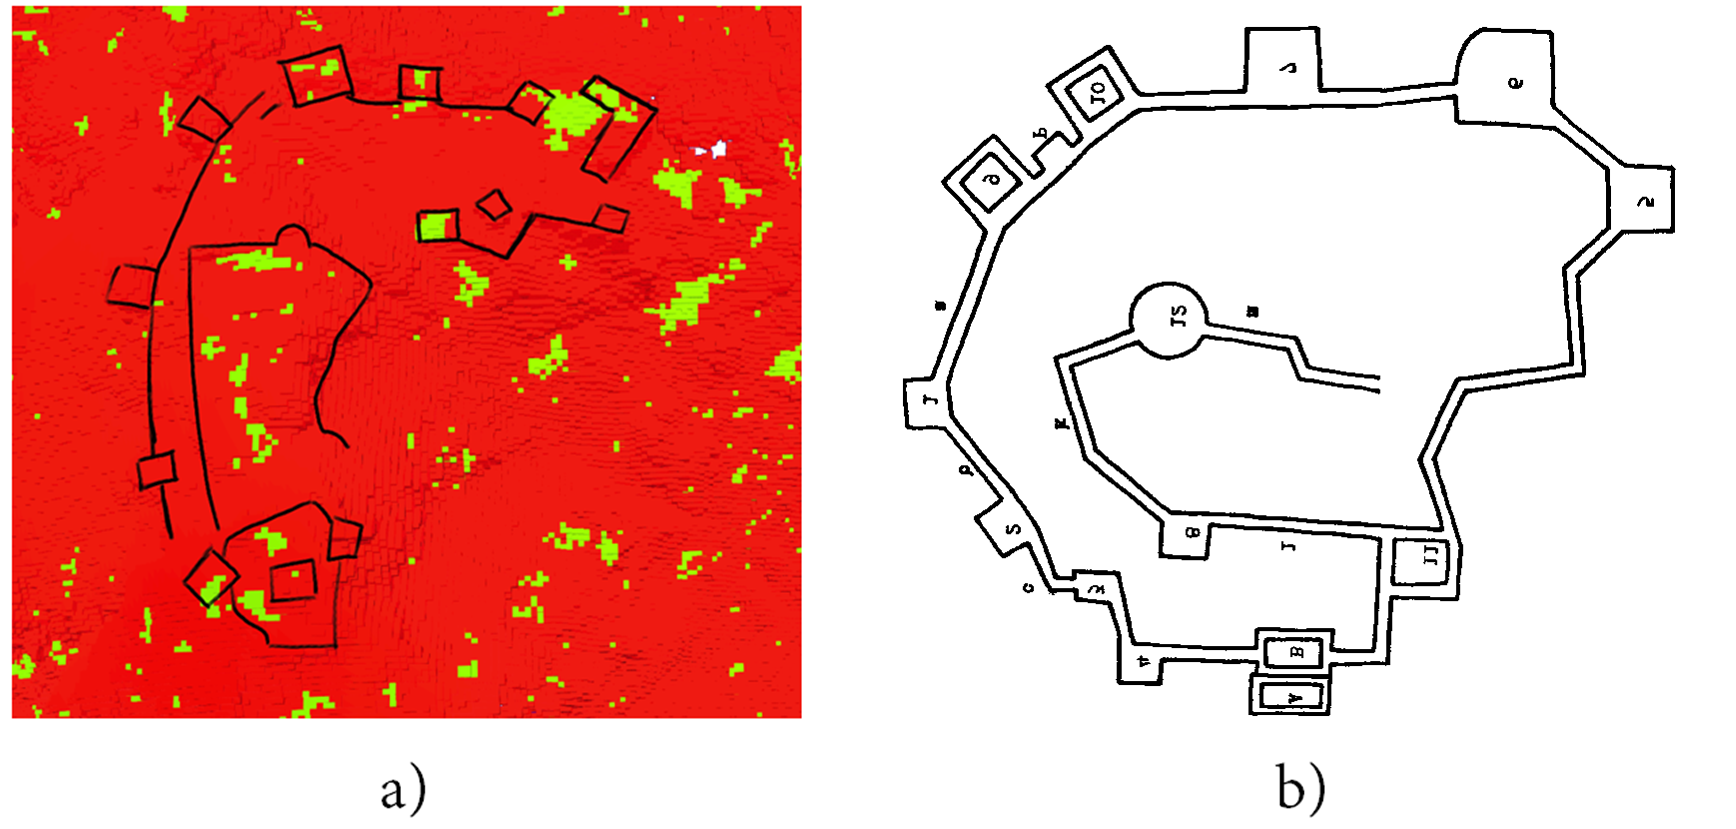
\includegraphics[width=.98\linewidth]{figs/castle_puerta_arenas/voxel_anomalies_highlighted.png}
	\caption{Comparison of a) anomalies detected from a 3D voxelized neighbourhood, depicting the underlying structure, and b) the enhanced structure proposed Fernández Hervás \cite{fernandez_hervas_castillo_1986}.}
	\label{fig:voxel_anomalies}
\end{figure}

% Principal results

\section{Experimental results and discussion}

This section is aimed at emphasizing some of the results that have been extracted from the aerial views. The following figures confirm some of the few conclusions drawn by previous literature circa 1990. The steep orography sculpted the shape of the fortress, fitting it to the contour of the hill. The castle has an 'L' shape ground plan where the short limb extends from the North to the West and the longest extends from North to South (see Figure \ref{fig:archaeological_remains_structure}). This configuration presents three defensive lines in the inner shape. 

\begin{figure}[htbp]
    \centering
    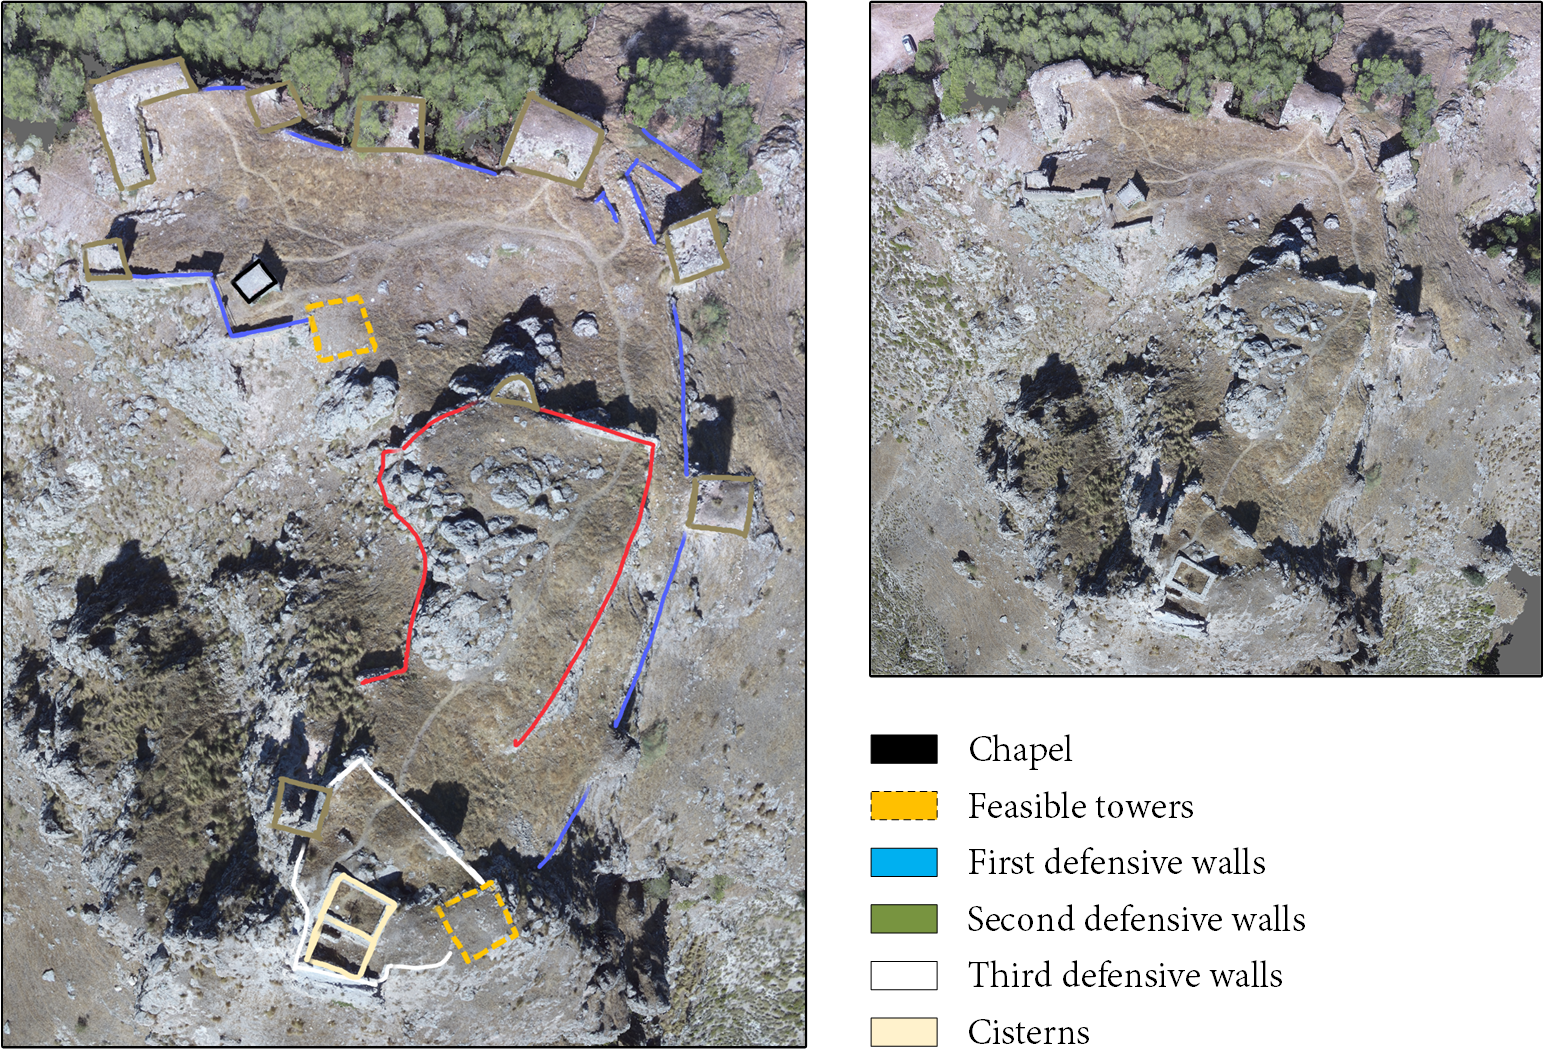
\includegraphics[width=\linewidth]{figs/castle_puerta_arenas/castle_annotations.png}
    \caption{Aerial view with highlighted archaeological remains, including both visible shapes and those identified with thermal imagery (dotted). }
    \label{fig:archaeological_remains_structure}
\end{figure}

The first defensive line is composed of the outermost walls, including the short limb as well as the boundaries of the longest. Therefore, it faces the cliff despite not reaching the southernmost part. On the other hand, the entrance located at the northernmost area of the outer wall is very poorly conserved. From the ground, there is only a clearly visible passage crossing two walls at an oblique angle (see Figure \ref{fig:entrance_details}). Additionally, the aerial views facilitate the finding of further remains that ought to be considered, despite going unnoticed in previous work. 

\begin{figure*}[htbp]
    \centering
    \includegraphics[width=\linewidth]{figs/castle_puerta_arenas/entrance_details.png}
    \caption{Fortress entrance in \acrshort{rgb} and thermal orthomosaics.}
    \label{fig:entrance_details}
\end{figure*}

The second defensive line presents another kind of tower and walls. This area is observed to be surrounded by the first defensive line on the North and East side. It faces the cliff on the West side as well as the third line on the South side. Only a tower seems to belong to this line: a semicircular tower built with big uncut stones. Note that cylindric towers were not usual in Arabic castles, and therefore it might be a construction of the later Christian settlement. Also, there seems to remain a water canalization system at the bottom of the tower, as depicted in Figure \ref{fig:water_sewer}.

\begin{marginfigure}[-2.0cm]
    \centering
    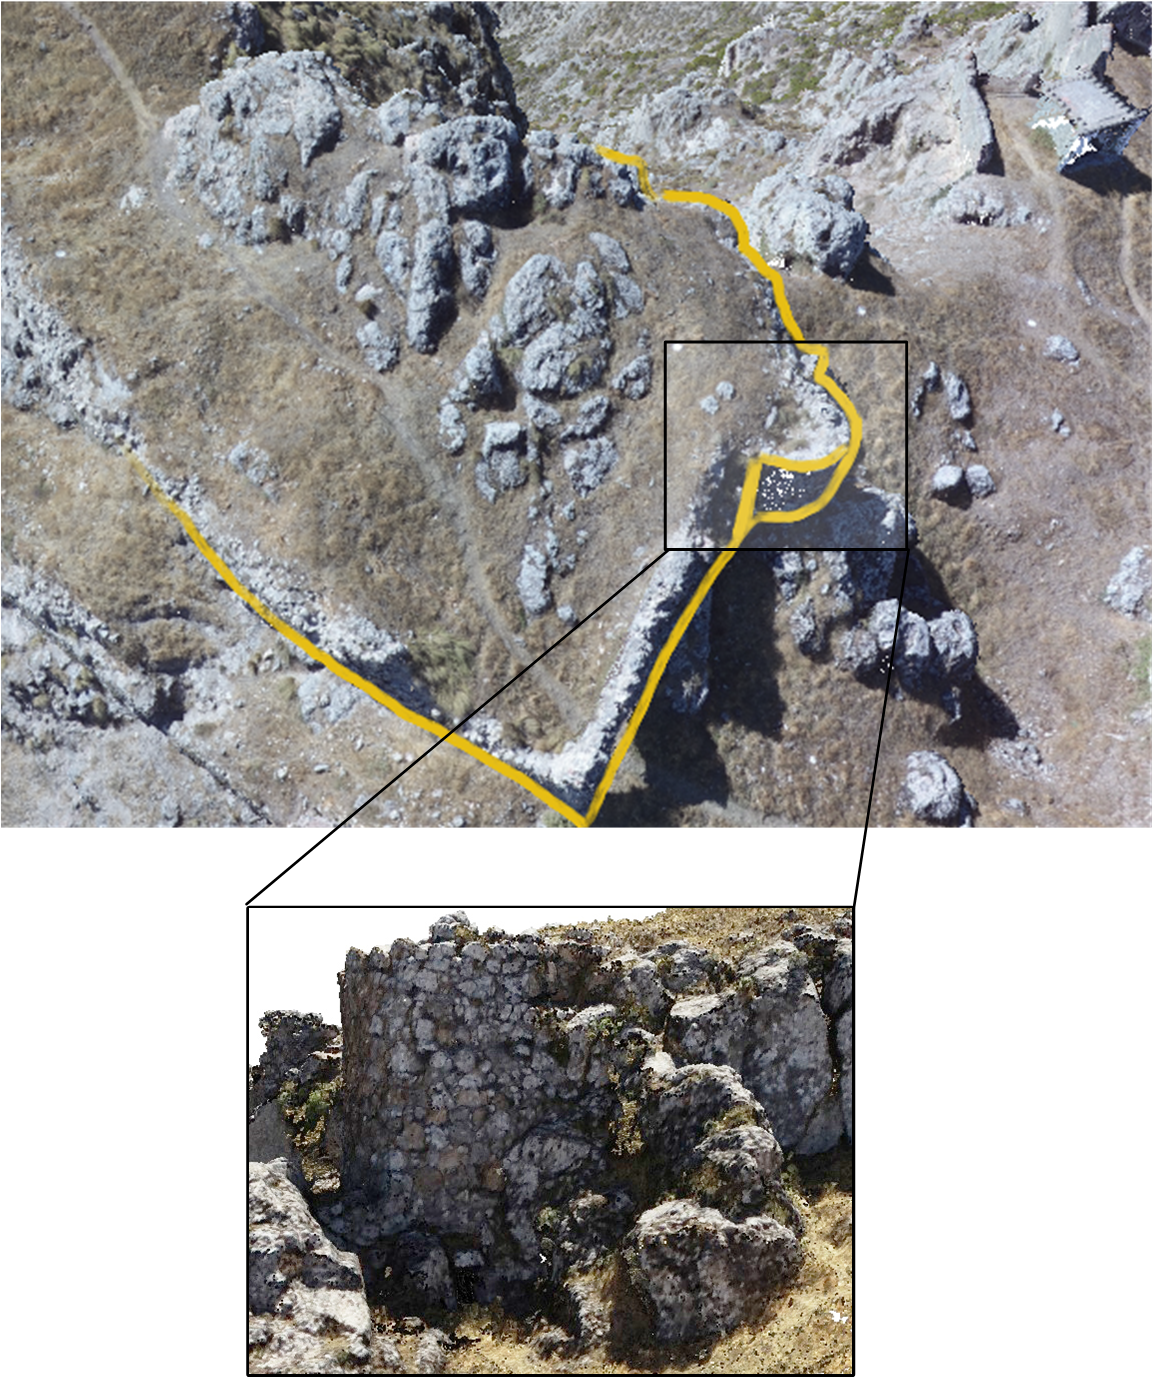
\includegraphics[width=\linewidth]{figs/castle_puerta_arenas/water_canalization.png}
	\caption{Water canalization system highlighted in the \acrshort{rgb} point cloud as well as its ground view.}
	\label{fig:water_sewer}
\end{marginfigure}

Between these defensive walls, there exists a flat space appropriate for the construction of smaller buildings. These are nowadays inaccessible due to the remains of the collapsed structures and sedimentation, and therefore, further surveys are required to provide better insight. In the thermal imagery, this zone is warmer than its surrounding area. Along with this, a more recent chapel was constructed at the end of the 19th century and rebuilt in recent years. In the long arm of the castle, right in front of the entrance, there is a huge pit with a width of 13 \si{\meter} and 4 \si{\meter} deep, which is supposed to be the result of plunder sometime between the abandonment and the declaration of the castle as a protected archaeological site. 

A third defensive line is composed of the walls in the southernmost area. It is also the most secure part of the fortress as it controls every side of the cliff but the North. It may be intended to join the middle walls to create a structure surrounded by several layers. The \acrshort{dem} in Figure \ref{fig:thermal_castle_dem} shows an anomalous geometry at the East side, with a similar size and shape to the West tower. However, it has steeper and more intricate access. The thermal imagery shows a noticeable anomaly in the same spot, as shown in Figure \ref{fig:cistern_tower}. With a minor ground survey, it was observed to be what seems like the basement of a tower. The fact that only the layout remains could be due to the strong winds that take place at the highest point of the hill. The existence of this tower may have passed unnoticed without aerial imagery. This area presents slopes near 50\% in the entrance passage, which along with its notable altitude \cite{modrego-fernandez_propuesta_2022}, makes this site hard to access and explore with ground-based surveys, such as \acrshort{tls}. The rest of the study area has a similar slope since it is located on a cliff. Therefore, \acrshort{uas} together with oblique flights has helped to collect images of every façade and observe subtle details.

\begin{figure*}[ht]
    \centering
    \includegraphics[width=\linewidth]{figs/castle_puerta_arenas/thermal_anomalies_3d.png}
    \caption{Rendering of thermal anomalies over two possible decimated towers. }
    \label{fig:cistern_tower}
\end{figure*}

Finally, there is another element that caught our attention: the water supply system. The orthomosaic shows two well-defined cisterns at the Southern part of the fortress, depicted as two contiguous rectangular shapes. There is also a small canalization that comes out of the middle wall, under the semicircular tower. It is similar to a small tunnel of a few tens of \si{\centi\meter}, though it follows a coarse canal made of rock in the first area and ends up at the cliff on the South side of the castle. Furthermore, previous work proposed the South side of the fortress as the location of two Arabic cisterns which may be the destination of the water flow.  
\section{Conclusions and future work}

The proposed procedure has led to the reconstruction of a 3D model with visible and infrared data, which can be later integrated into \acrshort{gis} and \acrshort{bim} projects, and can help archaeologists in the planning of excavations. Previous work addressing the fortress shape was performed with ground-based observations, whereas the extracted aerial view helps to develop a more precise idea of what the fortress looked like. The final products are represented in meters, thereby enabling the measurement of the dimensions of specific features, the distance among them, etc. Not only the visible remains were connected to provide a feasible structure, but also other abnormal areas were highlighted. These should be further investigated in future archaeological excavations. Furthermore, the objective after \acrshort{uas}, photogrammetry and thermal reconstructions is not only to shed light on ancient settlements but also to build a framework of preventive archaeology. Therefore, it helps in the preservation of cultural heritage and landscaping resources. 

Thermal imagery has been proven useful for detecting which areas should be excavated first to clarify how was the original structure. The 3D infrared reconstruction was performed over a dense \acrshort{rgb} point cloud, thus allowing us to visualize the study area with higher \acrshort{lod}. For instance, it helps to discard some anomalies caused by shadows. A semi-supervised automatic detection of anomalies was implemented over a 3D voxelization of the thermal point cloud. To this end, the temperature of each voxel was compared to its surroundings. Using this approach, some notable anomalies were detected near what is suspected to be two missing towers in the North and South area.   

In future work, more surveys should be conducted, even in night conditions, attending to the variations reflected in Figure \ref{fig:thermal_exchanging}. Also, a wider number of sensors could be used to provide more information, especially on those areas that are suspected to cover ancient remains. In this regard, magnetometry may shed some light to extract much more informed conclusions. Ground-based magnetometry may not be efficient due to the irregular and steep orography, whereas aerial magnetometry is more suitable for this case study. Even \acrshort{lidar} technology could be useful for obtaining surface microreliefs and therefore, spot places with buried remains. On the other hand, conventional methods, such as terrestrial photogrammetry, should only be used to provide complementary data sources with a higher \acrshort{lod} in specific areas.

\FloatBarrier
\section*{Additional data}

\renewcommand{\arraystretch}{1.2}
\begin{table*}[!htbp]
    \centering
    \caption{\acrshort{utm} coordinates (m) of \acrshort{gcp}s, as well as their East, North and height error in centimetres ($\delta_E$, $\delta_N$, $\delta_H$).}
    \label{table:point_coordinates}
    \begin{tabular}{llllllll}
    \toprule
    \multicolumn{8}{c}{\textbf{1) Control points}}\\
    \midrule
    Id & East $(\si{\metre})$ & North $(\si{\metre})$ & Height $(\si{\metre})$ & $\delta_E (\si{\centi\metre})$ & $\delta_N (\si{\centi\metre})$ & $\delta_H (\si{\centi\metre})$ & Total $\delta \hspace{1mm} (\si{\centi\metre})$\\
    \midrule
            1 & 444958.693 & 4160812.226 & 1342.189 & -0.4 & 0.5 & 2.3 & 2.4 \\
            2 & 444977.401 & 4160840.587 & 1341.810 & -1.5 & -0.5 & 1.3 & 2.0 \\
            3 & 445095.169 & 4160859.578 & 1357.320 & -0.2 & 0.4 & 0.6 & 0.7 \\
            4 & 445073.400 & 4160815.904 & 1374.452 & 2.0 & 0.2 & 1.7 & 2.6 \\
            5 & 445029.280 & 4160821.232 & 1375.903 & 1.2 & -1.5 & -2.2 & 2.9 \\
            7 & 445063.855 & 4160795.858 & 1383.090 & 1.1 & 0.2 & 0.3 & 1.2 \\
            9 & 445059.726 & 4160754.837 & 1389.440 & -1.9 & 0.8 & -0.2 & 2.1\\
    \midrule
    \multicolumn{4}{r}{\textbf{Absolute mean}} & \textbf{1.18} & \textbf{0.58} & \textbf{1.22} & \textbf{1.98} \\
    \midrule
    \multicolumn{8}{c}{\textbf{2) Checkpoints}}\\
    \midrule
    Id & E $(\si{\metre})$ & N $(\si{\metre})$ & H $(\si{\metre})$ & $\delta_E (\si{\centi\metre})$ & $\delta_N (\si{\centi\metre})$ & $\delta_H (\si{\centi\metre})$ & Total $\delta \hspace{1mm} (\si{\centi\metre})$\\
    \midrule
            6 & 445049.057 & 4160807.002 & 1376.097 & 6.0 & -9.4 & 3.8 & 11.8 \\
            8 & 445072.237 & 4160775.253 & 1383.474 & -1.6 & 2.0 & 8.0 & 8.4 \\
            10 & 445054.274 & 4160800.568 & 1378.135 & 2.9 & 3.8 & 9.9 & 11.0 \\
    \midrule
    \multicolumn{4}{r}{\textbf{Absolute mean}} & \textbf{3.5} & \textbf{5.06} & \textbf{7.23} & \textbf{10.4} \\
    \bottomrule
    \end{tabular}
    \normalsize
\end{table*}
\renewcommand{\arraystretch}{1}